

\begin{figure*}[!htbp]
	\begin{center}	\centerline{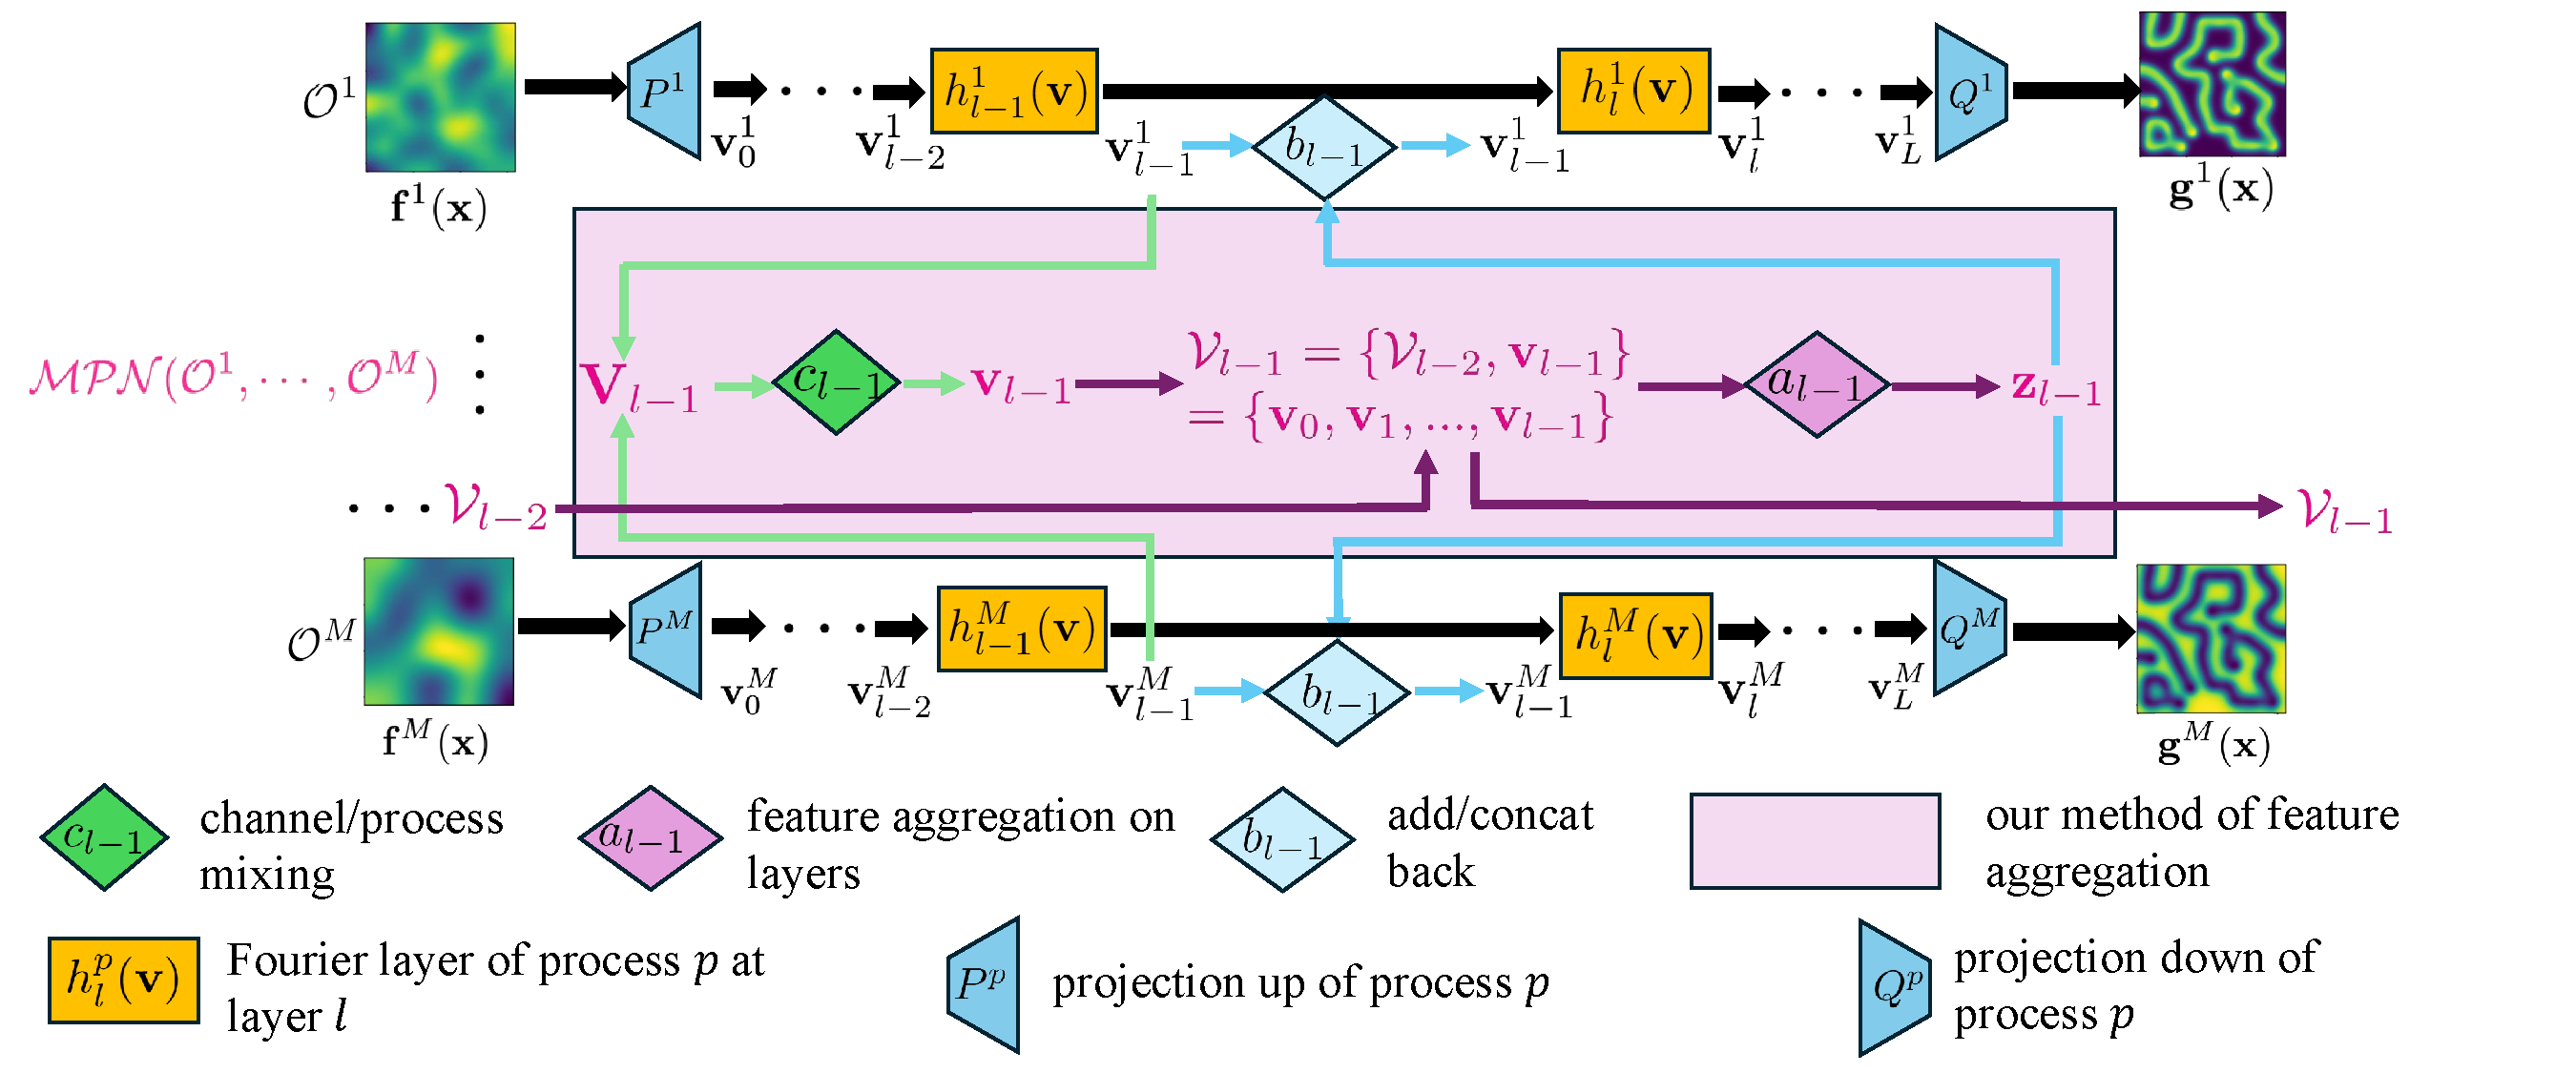
\includegraphics[width=1.0\textwidth]{figs/model2.pdf}}
        
		\caption{A graphical representation of \ours}
		\label{fig:model}
	\end{center}
    
\end{figure*}

%\vnegm
\section{Method}
%\vnegxxs
\subsection{Multi-Physics Simulation}
%\vnegxs
We consider multi-physics systems governed by \textit{coupled} partial differential equations (PDEs), which naturally emerge in diverse scientific and engineering disciplines, such as chemical reactions, environmental modeling, biological processes, and fluid mechanics. These systems involve multiple interacting physical processes, each described by its own PDE and interconnected through nonlinear coupling terms~\citep{weinan2003multiscale}. Such interactions substantially influence the overall system behavior, creating considerable modeling and computational challenges. Formally, a general mathematical representation for a coupled PDE system involving $M$ interacting physical processes is given by:

\begin{equation}
	\begin{aligned}
		\mathfrak{L}_m\left(u_1, u_2, \ldots, u_M\right)(x, t) & =f_m(x, t), \quad m=1, \ldots, M, \\
		u_m(x, t) & =0, \quad x \in \partial \Omega_m,
	\end{aligned}
\end{equation}

where $\mathfrak{L}_m$ represents differential operators, potentially including spatial and temporal derivatives and nonlinear terms capturing interactions among the physical processes. Here, $u_m(x,t)$ are the unknown state variables associated with the $m$-th physical process, and $f_m(x,t)$ represent known source terms, external inputs, or boundary conditions for each process.

%To illustrate this formulation clearly, consider a simple yet coupled PDE system such as the coupled reaction-diffusion system, commonly known as the Lotka-Volterra equations, used for modeling predator-prey dynamics:
%\begin{equation}
%	\begin{aligned}
%		& \frac{\partial u}{\partial t}=D_u \nabla^2 u+\alpha u-\beta u v, \\
%		& \frac{\partial v}{\partial t}=D_v \nabla^2 v+\delta u v-\gamma v,
%	\end{aligned}
%\end{equation}
%
%where $u(x,t)$ represents the prey population density, $v(x,t)$ represents the predator population density, and $D_u$, $D_v$ denote diffusion coefficients indicating the spatial spread of each species. The parameters $\alpha, \beta, \delta,$ and $\gamma$ represent the interaction rates such as growth, predation, and death. Each process evolves not only according to its own dynamics but also directly through interactions with other processes. Such interactions can lead to rich, emergent spatial-temporal patterns, making analytical solutions difficult or impossible, thus necessitating numerical or data-driven approaches for solution approximation.

%\vnegxxs
\subsection{Coupled Multi-Physics Operator Learning (\ours)}
%\vnegxs
Neural operator learning has shown great promise for modeling physical phenomena governed by PDEs. However, a significant limitation remains: most existing approaches assume that systems are governed by a single set of PDEs. This simplification overlooks the reality of physical simulations, where multiple processes interact across different scales, resulting in complex behaviors~\citep{keyes2013multiphysics}. Existing techniques like feature concatenation~\citep{wen2022u} and cross-overlaying~\citep{xiao2023coupled} attempt to model these interactions but are often insufficient for capturing sophisticated multi-physics scenarios.

To overcome this limitation, we propose \ours, a coupled multi-physics neural operator, $\mathcal{MPO}(\Ocal_1, \cdots, \Ocal_M)$ designed specifically to capture the intricate correlations among individual operators $\Ocal_1, \cdots, \Ocal_M$ of a multi-physics system. COMPOL achieves this by leveraging advanced neural operator architectures combined with sophisticated latent feature aggregation mechanisms. Formally, COMPOL approximates solution operators for coupled PDE systems as mappings between function spaces:
\[
	\mathcal{G}_\theta: \mathcal{H}_1 \times \mathcal{H}_2 \times \cdots \times \mathcal{H}_M \rightarrow \mathcal{Y}_1 \times \mathcal{Y}_2 \times \cdots \times \mathcal{Y}_M
\]
where each $\mathcal{H}_m$ denotes the function space of input functions (such as initial or boundary conditions), and $\mathcal{Y}_m$ denotes the corresponding output solution function space for the $m$-th physical process. Given input functions $f^m(x)$ representing the initial conditions or external inputs for each physical process, we first embed each process into a shared latent space to facilitate consistent interaction modeling:
\[
	v_0^m(x)=P^m\left(f^m(x)\right)
\]
where $P^m$ are linear projection operators mapping input functions into a common latent feature space, which enables unified treatment of heterogeneous processes. 

Subsequently, latent features undergo iterative transformations using nonlinear multi-physics neural operator layers explicitly designed to capture complex cross-process interaction:
\[
	v_l^m(x)=h_l^m\left(v_{l-1}^m(x), z_{l-1}(x)\right), \quad l=1, \ldots, L,
\]
where each neural operator layer $h_l^m$ comprises a nonlinear transformation that represents the internal process dynamics and is augmented by interaction-aware aggregated features $z_{l-1}(x)$. Specifically, the latent representation $v_l^m(x)$ captures the detailed inner-process transformations, encapsulating the \textit{process-specific} evolution and \textit{local dynamics} independently for each physical process. In contrast, the aggregated latent feature $z_{l-1}(x)$ explicitly represents \textit{inter-process} interactions, integrating \textit{global context} and information across different physical processes. This separation of inner-process transformations and inter-process interactions is a crucial design choice. It allows the model to independently refine representations of each process while simultaneously and explicitly modeling the intricate and nonlinear interactions among them.

The aggregated interaction features are computed using a carefully designed aggregation function:
\[
	z_{l-1}(x)=\mathcal{A}\left(v_{l-1}^1(x), v_{l-1}^2(x), \ldots, v_{l-1}^M(x)\right),
\]
with $\mathcal{A}(\cdot)$ denoting a specialized aggregation mechanism (such as recurrent or attention), ensuring coherent and effective representation of inter-process dependencies.

Finally, each process-specific solution is reconstructed from the latent features using dedicated linear projection operators:
%\[
%	g^m(x)=Q^m\left(v_L^m(x)\right), \quad Q^m: \mathbb{R}^{d_h} \rightarrow \mathbb{R}^{d_m},
%\]
\[
g^m(x)=Q^m\left(v_L^m(x)\right)
\]
yielding the predicted solutions $g^m(x)$ in their respective physical spaces.
%\vnegxxs
\paragraph{Universal Approximation Capabilities} COMPOL is theoretically grounded in the operator approximation theory, particularly relying on the universal approximation property of neural operator frameworks. According to this theory, neural operators can uniformly approximate any continuous nonlinear operator between Banach spaces. Specifically, given a continuous operator $\mathcal{G}: \mathcal{K}\subset\mathcal{H}\rightarrow\mathcal{Y}$ defined on a compact set $\mathcal{K}$, and for any $\varepsilon>0$, there exist neural operator parameters $\theta$ such that:
\[
	\sup _{f \in \mathcal{K}}\left\|\mathcal{G}(f)-\mathcal{G}_\theta(f)\right\|_y<\varepsilon .
\]
%\vnegxxs
\paragraph{Convergence of the Iterative Latent Transformation} In the context of COMPOL, the iterative transformations of latent representations can be interpreted as fixed-point iterative schemes:
\[
	v_l^m=\Phi_l^m\left(v_{l-1}^m, z_{l-1}\right), \quad z_{l-1}=\mathcal{A}\left(\left\{v_{l-1}^m\right\}_{m=1}^M\right),
\]

where $\Phi_l^m$ are nonlinear integral operators that encapsulate the process-specific inner transformations. Under appropriate conditions, such as Lipschitz continuity of $\Phi_l^m$ and $\mathcal{A}$, Banach’s fixed-point theorem ensures convergence to a unique fixed point, enhancing stability and reliability of the neural operator approximation.
%\vnegxxs
\paragraph{Stability of Latent Feature Aggregation} Moreover, the explicit distinction between inner-process transformations ($v_l^m$) and inter-process interactions ($z_l$) in COMPOL theoretically enhances expressivity and interpretability. The carefully designed aggregation mechanisms, such as gating in recurrent neural networks and adaptive weighting in attention mechanisms, provide structured inductive biases, facilitating robust and adaptive feature integration. These mechanisms inherently regularize the learning process and promote generalization by prioritizing and selectively integrating the most impactful cross-process interaction features. Thus, the explicit structural design of COMPOL offers a rigorous and theoretically justified approach for modeling complex multi-physics interactions.

Collectively, these theoretical results provide robust mathematical foundations for the COMPOL framework. The universal approximation theorem establishes that COMPOL can precisely model any complex multi-physics operator with arbitrary accuracy. The convergence theorem offers strong mathematical guarantees that COMPOL's iterative latent updates consistently converge, ensuring reliable and stable model predictions. Additionally, the stability theorem confirms that COMPOL robustly represents and integrates interactions between different physical processes, enhancing the interpretability and reliability of the learned latent representations. These rigorous theoretical underpinnings validate COMPOL's effectiveness, stability, and generalization capabilities when addressing complex, coupled multi-physics problems. We provide proofs in the Appendix \ref{sec:appx-proofs}.

%These theoretical results rigorously underpin COMPOL: the universal approximation theorem guarantees accurate modeling of arbitrary multi-physics operators, the convergence theorem ensures stable latent representation updates, and the stability theorem confirms robust inter-process interactions. Collectively, these results validate COMPOL’s effectiveness, interpretability, and generalization capabilities for complex multi-physics problems. Detailed proofs are provided in Appendix \ref{sec:appx-proofs}.
%\vnegxxs
\subsection{Aggregation of Multi-Physics Operator Layers}
%\vnegxs
We now restate the formulation explicitly using discretized function notation.  We consider a coupled physical system with $M$ processes, each associated with discretized input functions $\f^1, \dots, \f^M$ (Figure \ref{fig:model}). Each process $m$ first maps its input $\f^m$ to a latent representation $\v_0^m$ via a channel-wise linear layer $P^m: \mathbb{R}^{d_m}\rightarrow\mathbb{R}^{d_h}$, where $d_m$ and $d_h$ are input and latent dimensions, respectively. By stacking $L$ neural operator layers, each subsequent operator layer $h_l^m$ transforms latent representations $\v_{l-1}^m$ into $\v_l^m$. A final linear layer $Q^m: \mathbb{R}^{d_h}\rightarrow\mathbb{R}^{d_m}$ maps the latent representation $\v_L^m$ back to the output function $\g^m$. To capture inter-process interactions, we compute an aggregated latent state $\z_l=\mathcal{A}(\{\{\v^m_j\}_{m=1}^M\}_{j=0}^l)$ at each layer where aggregation mechanisms are implemented using either recurrent units~\citep{cho2014learning} or attention-based~\citep{vaswani2017attention} methods.
%\vnegxxs
\paragraph{Recurrent Aggregation State} For notational convenience, let $\Vcal$ represent the complete collection of intermediate latent features across $M$ processes and $L+1$ layers, where these features are produced by neural operator layers $\{\{h_l^m\}_{m=1}^M\}_{l=0}^L$. Specifically, $\Vcal = \{\{\v^m_l\}_{m=1}^M\}_{l=0}^L$. In the one-dimensional case, $\Vcal$ can be viewed as a $(L+1)\times M \times d_h$ tensor. From this structure, we define $\V_l$ as the $M \times d_h$ matrix obtained by extracting the $l$-th slice along the first dimension of $\Vcal$. We further introduce $\Vcal_{l}$ to represent the sequence of latent functions from layer $0$ through layer $l$, which can be written as $\Vcal_{l} = \{\V_j\}_{j=0}^{l}$. Within this notation, two cases are particularly noteworthy: $\V_0$ represents the collection of latent functions immediately following the channel-wise lifting operation, while $\V_L$ denotes the collection of all latent functions just before the channel-wise projection.

Our first attempt of computing the aggregation state of layer $l$ is with using Gated Recurrent Unit (GRU)~\citep{cho2014learning}, expressed as:
\begin{align}
	\q_l &= \sigma(\W_q\V_l + \U_q\z_{l-1} + \b_q) \notag\\
	\r_l &= \sigma(\W_r\V_l + \U_r\z_{l-1} + \b_r) \notag\\
	\tilde{\z_{l}} &= \text{tanh}(\W_z\V_l + \U_{z}(\r_l \odot \z_{l-1}) + \b_z)\notag\\
	\z_l &= \q_l \odot \z_{l-1} + (1 - \q_l) \odot \tilde{\z_{l}}\notag,
\end{align}
where, $\z_{l-1}$ represents the aggregation state from the previous layer, , $\V_l$ captures the collective latent transformations across all $M$ processes at layer $l$ and $\odot$ denotes element-wise multiplication. Computing the aggregation state $\z_l$ involves two intermediate states: the update gate $\q_l$, balancing historical and new information, and the reset gate $\r_l$, selectively filtering irrelevant past information. A candidate state $\tilde{\z}_l$ combines current inputs $\V_{l}$ with the filtered previous state $\r_l \odot \z_{l-1}$~\citep{jozefowicz2015empirical, pascanu2013construct}. The final aggregation state $\z_l$ is a weighted blend of $\z_{l-1}$ and $\tilde{\z}_l$ controlled by the update gate $\q_l$. This approach effectively captures intricate interactions across layers, enabling the model to leverage complex dynamics in the coupled physical system.


%\paragraph{Attention Aggregation State} Our second approach leverages attention mechanisms to compute the aggregation state $\z_l$, offering significant advantages over RNN-based methods ~\citep{bahdanau2014neural,vaswani2017attention} in capturing information from $\Vcal_l$. Unlike the sequential nature of RNNs, attention mechanisms process all elements simultaneously, assigning weights (attention scores) across $\Vcal_{l}$. This parallel processing enables $\z_l$ to dynamically focus on the most significant features within ${\V_1, \cdots, \V_l}$, providing a more versatile and computationally efficient framework for modeling interactions in the latent space of coupled multi-physics systems.
%
%The implementation begins with the application of channel-wise feed-forward neural networks $\Phi_{Q}$, $\Phi_{K}$, and $\Phi_{A}$, which transform $\Vcal_l$ into three distinct representations essential for computing attention scores: query ($\Qcal$), key ($\Kcal$), and value ($\Acal$). This transformation can be expressed as:
%
%\[
%\Qcal = \Phi_{Q}(\Vcal_{l}), \Kcal = \Phi_{K}(\Vcal_{l}), \Acal = \Phi_{A}(\Vcal_{l})
%\]
%The aggregation state at layer $l$, denoted as $\z_l$, is then computed through a weighted sum:
%
%\[
%\z_l = \sum_{k=1}^{l}\alpha_{lk}\A_{k}
%\]
%where $\A_{k}$ represents the $k$-th slice along the first dimension of $\Acal$. The attention weights $\alpha_{lk}$ are determined through a similarity-based computation:
%
%\[
%\alpha_{lk} = \frac{\exp(s_{lk})}{\sum_{j=1}^{l}\exp(s_{jk})}, s_{lk} = \frac{\Q_l \K_k^\top}{\sqrt{d_k}}
%\]
%where $\Q_l$ and $\K_k$ represent the $l$-th and $k$-th slices along the first dimension of $\Qcal$ and $\Kcal$ respectively.
%
%This attention mechanism determines feature importance by measuring similarities between $\Qcal$ and $\Kcal$ representations. The resulting attention scores quantify the relevance of each hidden state $\V_j$ (where $j\in 0,\cdots,l$) of $\Vcal_{l}$ to the current aggregation state $\z_l$. The final aggregation state is then computed by combining the value representations weighted by these attention scores. This approach enables $\z_l$ to intelligently focus on the most pertinent information, delivering a refined and adaptable method for feature aggregation in coupled multi-physics modeling.

%\vnegxxs
\paragraph{Attention Aggregation State} In the attention-based aggregation mechanism, we compute the global latent interaction state through a scaled dot-product attention tailored specifically for multi-physics systems. Initially, the latent features from each process are linearly projected into query ($Q$), key ($K$), and value ($A$) representations via process-specific transformations: $Q=\Phi_Q(\Vcal_l)$, $K=\Phi_K(\Vcal_l)$, and $A=\Phi_A(\Vcal_l)$. The aggregation state $\z_l$ is then derived as a weighted sum of these value vectors, where each weight $\alpha_j$ quantifies the significance of interactions involving the $j$-th process:
\[
z_l=\sum_{j=1}^M \alpha_j A_j, \quad \alpha_j=\frac{\exp \left(Q K_j^{\top} / \sqrt{d_k}\right)}{\sum_{i=1}^M \exp \left(Q K_i^{\top} / \sqrt{d_k}\right)},
\]
with $d_k$ representing the dimensionality of the key vectors. Thus, this approach explicitly encodes and integrates process-specific interactions, dynamically identifying and highlighting the most influential cross-process features at each layer.
%\vnegxxs
\paragraph{Complexity Analysis} The computational complexity of the COMPOL model includes three components. Projection layers have complexity $O(M  d_m  d_h)$, with $M$ processes, input dimension $d_m$, and latent dimension $d_h$. Each Fourier Neural Operator (FNO) layer involves FFT and inverse FFT operations, each with complexity $O(N \log N)$ per channel~\citep{cooley1965algorithm}, where $N$ denotes spatial discretization points, leading to a total complexity of $O(L  M  d_h \cdot N \log N)$ for $L$ layers. The aggregation mechanisms contribute additional complexity: $O(L  M^2  d_h)$ for attention-based aggregation and $O(L  M  d_h^2)$ for GRU-based aggregation. Overall, the complexity is dominated by the Fourier operations, $O(L  M  d_h \cdot N \log N)$, in typical scenarios where $N \log N \gg M, d_h$. Aggregation mechanisms significantly influence complexity only when $M$ or $d_h$ is exceptionally large.
%\vnegxxs
\paragraph{Generalizability to Other Neural Operator Frameworks} \ours builds upon the Fourier Neural Operator (FNO) due to its proven efficiency and strong performance across diverse tasks. Nonetheless, the proposed latent aggregation mechanisms are general and can be seamlessly integrated with other neural operator frameworks, such as DeepONet~\citep{lu2021learning}, GNO~\citep{li2020neural}, LNO~\citep{kovachki2023neural}, and transformer-based operators~\citep{wu2024transolver} (e.g., Transolver). We provide further discussion and illustrative implementations for extending COMPOL to these alternative frameworks in the Section \ref{sec:appx-adapting}.
%\vnegxxs
\paragraph{Scope and Limitations of COMPOL’s Applicability} \ours is designed specifically for neural operator frameworks that employ layer-wise latent transformations, a common feature among modern neural operator architectures. However, neural operators lacking this layer-wise structure cannot directly incorporate \ours’s aggregation mechanisms.
%\vnegxxs
\subsection{Training}
%\vnegxs
Given the training data that are simulated or sampled from a coupled multi-physics system, denoted as $\{\{\f_n^m, \y_n^m\}_{n=1}^{N_m}\}_{m=1}^M$, where $\f_n^m$ and $\y_n^m$ represent the $n$-th input and output functions, respectively, from the $m$-th process of the coupled system, we optimize our coupled multi-physics neural operator ($\mathcal{MPO}$) by minimizing the empirical risk,
\begin{align}
	\Lcal_{\mathcal{MPO}} = \EE_{m\sim\pi}\EE_{f^m\sim\mu^m}||\mathcal{MPO}(f)-y^m|| \notag \approx \frac{1}{M}\sum_{m=1}^M\frac{1}{N_m}\sum_{n=1}^{N_m}||\g^m_n-\y_n^m||\notag,
\end{align}
where $\g_n^m$ is the prediction of $\f^m_n$. We can then use any gradient-based optimization method to minimize $\Lcal_{\mathcal{MPO}}$.
















